\documentclass[tikz,border=6pt]{standalone}
\usepackage{pgf-umlcd}
\begin{document}
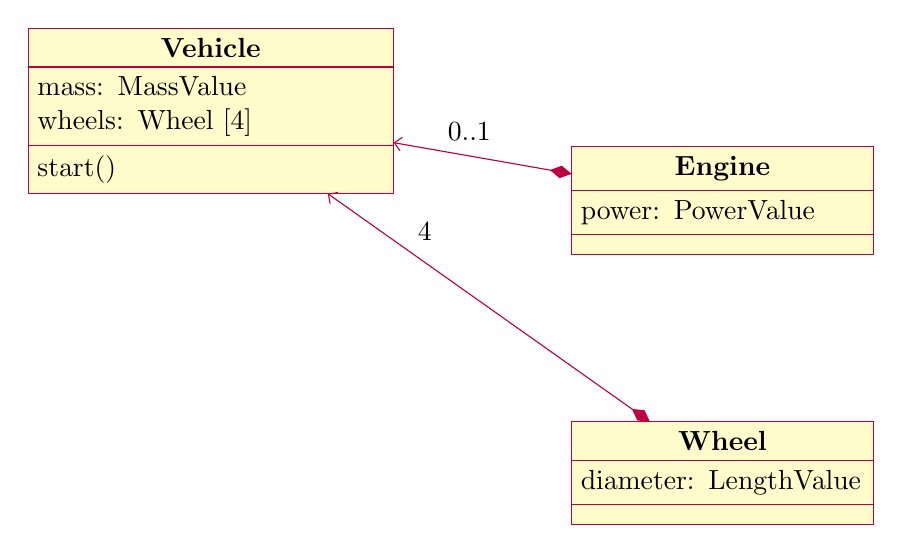
\begin{tikzpicture}
  \begin{class}[text width=4.4cm]{Vehicle}{0,0}
    \attribute{mass: MassValue}
    \attribute{wheels: Wheel [4]}
    \operation{start()}
  \end{class}

  \begin{class}[text width=3.6cm]{Engine}{6.5,-1.5}
    \attribute{power: PowerValue}
  \end{class}

  \begin{class}[text width=3.6cm]{Wheel}{6.5,-5.0}
    \attribute{diameter: LengthValue}
  \end{class}

  \composition{Engine}{}{0..1}{Vehicle}{}{1}
  \composition{Wheel}{}{4}{Vehicle}{}{1}
\end{tikzpicture}
\end{document}
